% L6b_Stability.pdf
\providecommand{\modre}[1]{\textcolor{NavyBlue}{#1}}
\providecommand{\cervene}[1]{\textcolor{Red}{#1}}
\providecommand{\zelene}[1]{\textcolor{OliveGreen}{#1}}
\providecommand{\dbar}{{\mathchar'26\mkern-12mu d}}

\section{Podmínky stability}
\strana{L6b-1}
\begin{itemize}
  \item termodynamická rovnováha musí být stabilní, jinak by systém mohl rovnovážný stav samovolně opustit
  \[
    \Rightarrow\quad \delta S = 0 \quad\&\quad \vzorec{\delta^2S < 0}
  \]
  \item výše uvedené variace bereme vůči \uv{volným} vnitřním parametrům složeného systému, ukážeme však, že stabilita vůči fluktuacím vyžaduje obecnou konkávnost fund.\ rovnice $S = S(U,\vec X)$ pro každý jednoduchý (pod)systém
  \item důsledkem nestability jsou např.\ \underline{fázové přechody}
\end{itemize}

\begin{priklad}[Př:]
\begin{minipage}{0.55\textwidth}
\begin{tikzpicture}[scale=0.95]
  \draw[->] (-0.3,0) -- (5.6,0) node[below right] {$U$};
  \draw[->] (0,-0.2) -- (0,4.4) node[left] {$S$};
  % konvexní křivka S(U)
  \draw[thick] (0.3,0.25) .. controls (1.5,0.35) and (2.7,0.6) .. (3.4,1.2)
                .. controls (3.9,1.7) and (4.3,2.6) .. (4.5,4.3);
  % body
  \coordinate (A) at (2.4,0.55);
  \coordinate (B) at (3.4,1.2);
  \coordinate (C) at (4.3,3.0);
  \fill (A) circle (1.5pt);
  \fill (C) circle (1.5pt);
  \fill[OliveGreen] (B) circle (2pt);
  % sečna
  \draw[dashed] ($(A)!-0.3!(C)$) -- ($(A)!1.3!(C)$);
  \fill[Red] (3.4,1.83) circle (2pt);
  % pomocné čáry
  \draw[dashed] (0,0.55) -- (A) -- (2.4,0);
  \draw[dashed] (0,1.2) -- (B) -- (3.4,0);
  \draw[dashed] (0,1.83) -- (3.4,1.83);
  \draw[dashed] (0,3.0) -- (C) -- (4.3,0);
  \node[below] at (2.4,0) {\small $U-\Delta U$};
  \node[below] at (3.4,-0.05) {\small $U$};
  \node[below] at (4.5,0) {\small $U+\Delta U$};
  \node[left,Red] at (0,1.83) {$S_\Delta$};
  \node[left,OliveGreen] at (0,1.2) {$S_{eq}$};
\end{tikzpicture}
\end{minipage}
\begin{minipage}{0.43\textwidth}
$\bullet$ mějme 2 identické podsystémy $\Rightarrow$
\[ S_{tot} = \sum_i S(U_i,V_i,N_i) \]
\begin{flushright}
$U, V, N$ \\
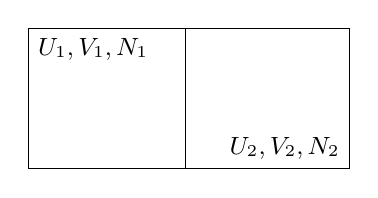
\begin{tikzpicture}[scale=0.85]
  \draw (0,0) rectangle (4.8,2.1);
  \draw (2.35,0) -- (2.35,2.1);
  \node[anchor=north west] at (0,2.1) {\small $U_1,V_1,N_1$};
  \node[anchor=south east] at (4.8,0) {\small $U_2,V_2,N_2$};
\end{tikzpicture}
\end{flushright}
\end{minipage}

\begin{itemize}
  \item rovnováha: \quad $U_1 = U_2 = U$, \ $V_1 = V_2 = V$, \dots \\
        $\Rightarrow$ \ $S_{eq} = 2S(U,V,N)$ \ \zelene{$\Leftrightarrow\ \bullet$}
  \item fluktuace: \quad $U\to U + \Delta U$ v 1 části $\Leftrightarrow$ $U\to U - \Delta U$ ve 2. \\
        $\Rightarrow$ \ $S_\Delta = S(U+\Delta U,V,N) + S(U-\Delta U,V,N)$ \ \cervene{$\Leftrightarrow\ \bullet$}
\end{itemize}
\[
  \Rightarrow\ \cervene{S_\Delta} > \zelene{S_{eq}} \ \text{pro konvexní } S \ \Rightarrow\
  \text{systém má tendenci k vnitřním nehomogenitám\,\pozor{!}}
\]
\hspace*{4cm}$\Rightarrow$ domény různých fází
\end{priklad}

%----------------------------------------------------------------------
\strana{L6b-2}
\begin{itemize}
  \item \underline{entropie stabilního systému} (tedy mimo oblasti fáz.\ přechodů) musí být \underline{konkávní}
\end{itemize}
\[
  S(U+\Delta U,V,N) + S(U-\Delta U,V,N) - 2S(U,V,N) \leq 0
\]
\begin{minipage}{0.4\textwidth}
\[
  \Big\downarrow\ \Delta U\to 0
\]
\[
  \left(\frac{\partial^2S}{\partial U^2}\right)_{V,N} \leq 0
\]
\end{minipage}
\begin{minipage}{0.58\textwidth}
\modre{$\nearrow\ -\dfrac{1}{T^2}\left(\pdv{T}{U}\right)_{V,N} = -\dfrac{1}{T^2C_V} \leq 0 \ \Rightarrow\ C_V \geq 0$}

\medskip
\end{minipage}
\[
  \zelene{\frac{\dd^2f}{\dd x^2} = \lim_{h\to0}\frac{\frac{f(x+h)-f(x)}{h} - \frac{f(x)-f(x-h)}{h}}{h} = \lim_{h\to0}\frac{f(x+h) - 2f(x) + f(x-h)}{h^2}}
\]

$\to$ analog.\ úvaha vede na \quad $\left(\dfrac{\partial^2S}{\partial V^2}\right)_{U,N} \leq 0$, \dots \hfill \modre{VIZ STR.\ 7}

$\Rightarrow$ obecně dostávám podmínku na negativní definitnost kvadratické formy
\begin{veta}[Podmínka stability]
\[
  \vzorec{\delta^2S = \frac12\sum_{i,j}\left(\frac{\partial^2S}{\partial X_i\,\partial X_j}\right)\delta X_i\,\delta X_j \leq 0}
\]
\hfill ($X_i$ zahrnuje $\forall$ ext.\ param.\ vč.\ $U$)
\end{veta}

\noindent\rule{\linewidth}{0.4pt}

Počítejme \\
$\delta_{\vec X^1}S$ pro $S = S_1(\vec X^1) + S_2(\vec X - \vec X^1)$; jsme-li v rovnováze, pak tato \uv{fluktuace} musí být záporná ($S$ je vzhledem k $\vec X^1$ již v maximu)
\[
  \underset{\substack{\uparrow\\ \text{Taylor: } S(\vec x) = S(\vec x_0) + \dd_hS + \frac{1}{2!}\dd_h^2S + \cdots}}{\delta S}
  = \left(\pdv{S}{X_i^1}\right)\delta(X_i^1) + \frac{1}{2!}\,\delta X_i^1\left(\frac{\partial^2S}{\partial X_i^1\,\partial X_j^1}\right)\delta X_j^1
\]
\begin{align*}
  &= \underbrace{\left[\left(\pdv{S_1}{X_i^1}\right) - \left(\pdv{S_2}{X_i^2}\right)\right]}_{=0\ \text{v rovnováze}}\delta X_i^1
   + \frac12\,\delta X_i^1\left[\left(\frac{\partial^2S_1}{\partial X_i^1\,\partial X_j^1}\right) + \left(\frac{\partial^2S_2}{\partial X_i^2\,\partial X_j^2}\right)\right]\delta X_j^1 \\
  &= \frac12\,\delta X_i^1\left[\left(\frac{\partial^2S_1}{\partial X_i^1\,\partial X_j^1}\right) + \left(\frac{\partial^2S_2}{\partial X_i^2\,\partial X_j^2}\right)\right]\delta X_j^1 \leq 0
\end{align*}

%----------------------------------------------------------------------
\strana{L6b-3}
$\Rightarrow$ pro \underline{identické podsystémy}
\[
  \delta^2S = \delta X_i\left(\frac{\partial^2S}{\partial X_i\,\partial X_j}\right)\delta X_j \leq 0
  \ \Leftrightarrow\ \text{\parbox[t]{5cm}{druhý diferenciál je negativně (semi)def.\ forma}}
\]
\cervene{\textbf{!} Zde se již jedná o druhou variaci/diferenciál vůči \underline{všem extenzivním proměnným} (tj.\ $U$ a deformační souřadnice) \underline{jednoduchého systému}\,\textbf{!}}

\begin{itemize}
  \item \underline{semi}: $\Leftarrow$ 1) extenzivita \\
        \phantom{\underline{semi}:} $\Leftarrow$ 2) fázové přechody (oblasti loc.\ nestability)
\end{itemize}

\underline{Nb:} \quad $\delta^2S = -\dfrac1T\,\delta^2U$ \quad \& \quad $\delta^2U = \delta T\,\delta S + \sum_{i=1}^{k}\delta y_i\,\delta X_i$

$\Rightarrow$ dostáváme \underline{obecnou podmínku stability}
\begin{veta}[Obecná podmínka stability]
\[
  \delta^2U = \vzorec{\delta T\,\delta S + \sum_{i=1}^{k}\delta y_i\,\delta X_i = \delta T\,\delta S - \delta p\,\delta V + \delta\mu\,\delta N > 0}
\]
\quad $\bullet$ $\forall$ variace samozřejmě nejsou nezávislé\,\pozor{!}
\end{veta}

\modre{
\begin{itemize}
  \item z odvození plyne, že tato podmínka se vztahuje k (entropické) fund.\ rovnici jako takové než k fluktuacím příslušného (izolovaného!) systému v rovnováze
\end{itemize}
$\Rightarrow$ $\delta^2S \leq 0$ platí pro každý podsystém zvlášť, přestože $\delta S\neq 0$!}

\begin{center}
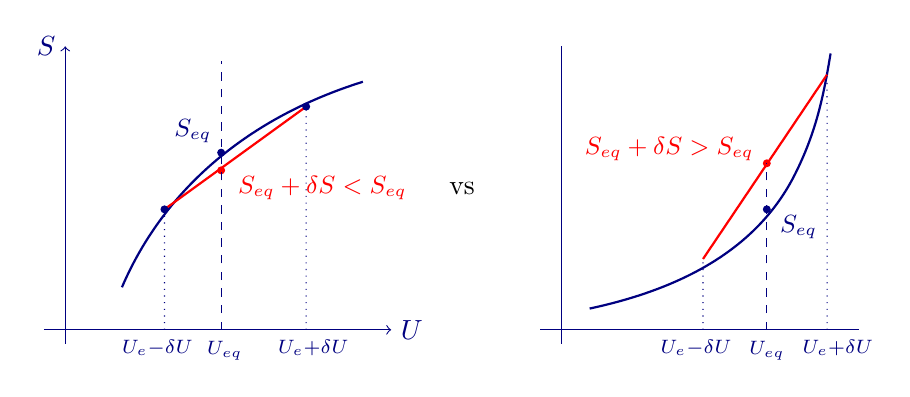
\begin{tikzpicture}[scale=0.9,NavyBlue]
  % levý (konkávní)
  \draw[->] (0,-0.2) -- (0,4) node[left] {$S$};
  \draw[->] (-0.3,0) -- (4.6,0) node[right] {$U$};
  \draw[thick] (0.8,0.6) .. controls (1.4,2.0) and (2.6,3.0) .. (4.2,3.5);
  \coordinate (L1) at (1.4,1.7);
  \coordinate (L2) at (2.2,2.5);
  \coordinate (L3) at (3.4,3.15);
  \draw[Red,thick] (L1) -- (L3);
  \fill (L1) circle (1.6pt) (L3) circle (1.6pt);
  \fill (L2) circle (1.6pt);
  \fill[Red] (2.2,2.25) circle (1.6pt);
  \draw[dashed] (2.2,0) -- (2.2,3.8);
  \draw[dotted] (1.4,0) -- (L1);
  \draw[dotted] (3.4,0) -- (L3);
  \node[above left] at (L2) {\small $S_{eq}$};
  \node[Red,right] at (2.3,2.0) {\small $S_{eq}+\delta S < S_{eq}$};
  \node[below] at (1.3,0) {\scriptsize $U_e{-}\delta U$};
  \node[below] at (2.25,-0.02) {\scriptsize $U_{eq}$};
  \node[below] at (3.5,0) {\scriptsize $U_e{+}\delta U$};
  \node[black] at (5.6,2) {vs};
  % pravý (konvexní)
  \begin{scope}[xshift=7cm]
    \draw (0,-0.2) -- (0,4);
    \draw (-0.3,0) -- (4.2,0);
    \draw[thick] (0.4,0.3) .. controls (1.8,0.6) and (2.8,1.2) .. (3.3,2.2) .. controls (3.6,2.8) and (3.7,3.3) .. (3.8,3.9);
    \coordinate (R1) at (2.0,1.0);
    \coordinate (R2) at (2.9,1.7);
    \coordinate (R3) at (3.75,3.6);
    \draw[Red,thick] (R1) -- (R3);
    \fill (R2) circle (1.6pt);
    \fill[Red] (2.9,2.35) circle (1.6pt);
    \draw[dashed] (2.9,0) -- (2.9,2.35);
    \draw[dotted] (2.0,0) -- (R1);
    \draw[dotted] (3.75,0) -- (R3);
    \node[Red,left] at (2.85,2.55) {\small $S_{eq}+\delta S > S_{eq}$};
    \node[right] at (2.95,1.45) {\small $S_{eq}$};
    \node[below] at (1.9,0) {\scriptsize $U_e{-}\delta U$};
    \node[below] at (2.9,-0.02) {\scriptsize $U_{eq}$};
    \node[below] at (3.9,0) {\scriptsize $U_e{+}\delta U$};
  \end{scope}
\end{tikzpicture}
\end{center}

%----------------------------------------------------------------------
\strana{L6b-4}
\begin{itemize}
  \item nyní konkrétní volbou nezávislých variací a aplikací MR odvodíme různé fundamentální podmínky pro koeficienty lin.\ odezvy
\end{itemize}

\begin{priklad}[A) $\delta T, \delta p, \delta N$ nezávislé \ {\normalfont ($\leftrightarrow$ Gibbsovské proměnné)}]
\begin{align*}
  \delta S &= \left(\pdv{S}{T}\right)_{p,N}\delta T + \left(\pdv{S}{p}\right)_{T,N}\delta p + \left(\pdv{S}{N}\right)_{T,p}\delta N && \modre{\times\,\delta T} \\
  \delta V &= \left(\pdv{V}{T}\right)_{p,N}\delta T + \left(\pdv{V}{p}\right)_{T,N}\delta p + \left(\pdv{V}{N}\right)_{T,p}\delta N && \modre{\times\,\delta p} \\
  \delta\mu &= \left(\pdv{\mu}{T}\right)_{p,N}\delta T + \left(\pdv{\mu}{p}\right)_{T,N}\delta p + \left(\pdv{\mu}{N}\right)_{p,T}\delta N && \modre{\times\,\delta N}
\end{align*}
\begin{align*}
  \Rightarrow\ \delta T\,\delta S - \delta p\,\delta V + \delta\mu\,\delta N &= \left(\pdv{S}{T}\right)_{p,N}(\delta T)^2 \\
  &\quad + \delta T\,\delta p\left[\left(\pdv{S}{p}\right)_{T,N} - \left(\pdv{V}{T}\right)_{p,N}\right]
   + \delta T\,\delta N\left[\left(\pdv{S}{N}\right)_{T,p} + \left(\pdv{\mu}{T}\right)_{p,N}\right] \\
  &\quad - (\delta p)^2\left(\pdv{V}{p}\right)_{T,N} + \delta p\,\delta N\left[-\left(\pdv{V}{N}\right)_{T,p} + \left(\pdv{\mu}{p}\right)_{T,N}\right] \\
  &\quad + (\delta N)^2\left(\pdv{\mu}{N}\right)_{p,T} \ \geq 0
\end{align*}
\underline{MR:} \quad $\dd G = -S\,\dd T + V\,\dd p + \mu\,\dd N$ \ $\Rightarrow$
\begin{enumerate}[label=\arabic*)]
  \item $\delta T\,\delta p\,[\ ] = -2\alpha V\,\delta T\,\delta p$
  \item $[\ ]$ u ostatních smíš.\ variací $= 0$
\end{enumerate}
\[
  \Rightarrow\ \left(\pdv{S}{T}\right)_{p,N}(\delta T)^2 - 2\alpha V\,\delta T\,\delta p - \left(\pdv{V}{p}\right)_{T,N}(\delta p)^2 + \left(\pdv{\mu}{N}\right)_{p,T}(\delta N)^2 \geq 0
\]
\[
  \Rightarrow\ \frac{C_p}{T}(\delta T)^2 - 2V\alpha\,\delta T\,\delta p + V\kappa_T(\delta p)^2 + \left(\pdv{\mu}{N}\right)_{p,T}(\delta N)^2 \geq 0
\]
\[
  \modre{(\delta T\ \delta p\ \delta N)
  \begin{pmatrix} C_p/T & -V\alpha & 0 \\ -V\alpha & V\kappa_T & 0 \\ 0 & 0 & \left(\frac{\partial\mu}{\partial N}\right)\end{pmatrix}
  \begin{pmatrix}\delta T\\ \delta p\\ \delta N\end{pmatrix} > 0}
\]
\end{priklad}

%----------------------------------------------------------------------
\strana{L6b-5}
$\Rightarrow$ \underline{Sylvester}: \quad \parbox[t]{0.75\textwidth}{
$\bullet$ \ $\vzorec{C_p \geq 0}$ \\[3pt]
$\bullet$ \ $\dfrac{C_pV\kappa_T}{T} - V^2\alpha^2 \geq 0 \ \Rightarrow\ C_p\kappa_T \geq TV\alpha^2 \ \Rightarrow\ \vzorec{\kappa_T \geq 0}$ \\[3pt]
$\bullet$ \ $\vzorec{\left(\pdv{\mu}{N}\right)_{T,p} \geq 0}$}

\quad {\small $\uparrow$ $\forall$ minory kvadr.\ formy pozitivní}

\underline{NB:} Meyerův vztah \quad $\underline{C_V = C_p - TV\dfrac{\alpha^2}{\kappa_T} \geq 0}$ \quad (plyne z druhé podmínky)

\begin{priklad}[B) $T, V, N$ nezávislé]
$\bullet$ stejným postupem:
\begin{align*}
  0 \leq \delta S\,\delta T - \delta p\,\delta V + \delta\mu\,\delta N
  &= \left(\pdv{S}{T}\right)_{V,N}(\delta T)^2 - \left(\pdv{p}{V}\right)_{T,N}(\delta V)^2
   + \left(\pdv{\mu}{N}\right)_{T,V}(\delta N)^2 \\
  &\quad + \left[\left(\pdv{S}{V}\right)_{T,N} - \left(\pdv{p}{T}\right)_{V,N}\right]\delta V\,\delta T \\
  &\quad + \left[\left(\pdv{S}{N}\right)_{T,V} + \left(\pdv{\mu}{T}\right)_{V,N}\right]\delta T\,\delta N \\
  &\quad + \left[\left(\pdv{\mu}{V}\right)_{T,N} - \left(\pdv{p}{N}\right)_{T,V}\right]\delta V\,\delta N \geq 0
\end{align*}
$\bullet$ $\dd F = -S\,\dd T - p\,\dd V + \mu\,\dd N$ \\
\quad $\Rightarrow$ $\delta V\,\delta T$ vypadne \\
\quad $\Rightarrow$ $\delta T\,\delta N$ vypadne \quad \& \quad
$\left(\pdv{\mu}{V}\right)_{T,N} = -\left(\pdv{p}{N}\right)_{T,V} = \dfrac{\left(\pdv{V}{N}\right)_{T,p}}{\left(\pdv{V}{p}\right)_{T,N}}$
\[
  \Rightarrow\ \frac{C_V}{T}(\delta T)^2 + \frac{1}{V\kappa_T}(\delta V)^2 + \left(\pdv{\mu}{N}\right)_{T,V}(\delta N)^2 - 2\left(\pdv{p}{N}\right)_{T,V}\delta V\,\delta N \geq 0
\]
\[
  \Rightarrow\ \frac{C_V}{T}(\delta T)^2 + \frac{1}{V\kappa_T}(\delta V)^2 + \left(\pdv{\mu}{N}\right)_{T,V}(\delta N)^2 + 2\,\frac{\left(\pdv{V}{N}\right)_{T,p}}{V\kappa_T}\,\delta V\,\delta N \geq 0
\]
\[
  \dd G = -S\,\dd T + V\,\dd p + \mu\,\dd N \ \Rightarrow\ \left(\pdv{V}{N}\right)_{T,p} = \left(\pdv{\mu}{p}\right)_{T,N}
\]
\end{priklad}

%----------------------------------------------------------------------
\strana{L6b-6}
\begin{minipage}[t]{0.42\textwidth}
\begin{veta}[Podmínky stability (B)]
$\Rightarrow$
\begin{tabular}{l@{\qquad}l}
$\bullet$ $\vzorec{C_V > 0}$ & $(\delta T)^2$ \\[4pt]
$\bullet$ $\vzorec{\kappa_T > 0}$ & $(\delta V)^2$ \\[4pt]
$\bullet$ $\left(\pdv{\mu}{N}\right)_{T,V} > 0$ & $(\delta N)^2$
\end{tabular}
\end{veta}
\end{minipage}\hfill
\begin{minipage}[t]{0.55\textwidth}
\small
\[
  (\delta V,\delta N)\begin{pmatrix}\frac{1}{V\kappa_T} & -\left(\frac{\partial p}{\partial N}\right)\\ -\left(\frac{\partial p}{\partial N}\right) & \left(\frac{\partial\mu}{\partial N}\right)\end{pmatrix}(\delta V,\delta N)
\]
\[
  = (\delta V,\delta N)\begin{pmatrix}\frac{\delta V}{V\kappa_T} - \left(\frac{\partial p}{\partial N}\right)\delta N \\ -\left(\frac{\partial p}{\partial N}\right)\delta V + \left(\frac{\partial\mu}{\partial N}\right)\delta N\end{pmatrix} \ \checkmark
\]
\end{minipage}

{\small
\[
  \Rightarrow\ \frac{\left(\frac{\partial\mu}{\partial N}\right)_{T,V}}{V\kappa_T} - \left[\left(\pdv{p}{N}\right)_{T,V}\right]^2 > 0
\]
\[
  \Rightarrow\ \left[\left(\pdv{p}{N}\right)_{T,V}\right]^2 = \left(\frac{\left(\frac{\partial V}{\partial N}\right)_{T,p}}{V\kappa_T}\right)^2
  = \left[\frac{\left(\frac{\partial\mu}{\partial p}\right)_{T,N}}{V\kappa_T}\right]^2 < \frac{\left(\frac{\partial\mu}{\partial N}\right)_{T,V}}{V\kappa_T}
\]
\[
  \Rightarrow\ \frac{1}{V\kappa_T}\left[\left(\pdv{V}{N}\right)_{T,p}\right]^2 < \left(\pdv{\mu}{N}\right)_{T,V}
  \quad\&\quad
  \frac{1}{V\kappa_T}\left(\pdv{\mu}{p}\right)_{T,N}^2 < \left(\pdv{\mu}{N}\right)_{T,V}
\]
\hfill $\Rightarrow$ nic relevantního}

\underline{NB:} \modre{sklon adiabaty a izotermy} -- víme \ $\dfrac{\kappa_S}{\kappa_T} = \dfrac{C_V}{C_p}$ \quad $\Rightarrow$ \quad
$\vzorec{\kappa_S = -\frac1V\left(\pdv{V}{p}\right)_S > 0}$

\subsection{Termodynamické potenciály -- alternativní formulace}
\begin{itemize}
  \item z vlastností Leg.\ transformací vyplývá, že je-li $U(X_1,\dots,X_{k+1})$ konvexní ve $\forall$ ext.\ proměnných $X_i$, potom
  \[ P = U[y_1,\dots,y_m](y_1,\dots,y_m,X_{m+1},\dots,X_{k+1}) \]
  je \kw{konkávní} v $y_1,\dots,y_m$ a \kw{konvexní} v $X_{m+1},\dots,X_{k+1}$
  \item přesněji (viz dodatek)
  \[
    U = P + \sum_{i=1}^{m}y_iX_i
  \]
  \[
    \Rightarrow\ \delta^2U = -\sum_{i,j=1}^{m}\delta y_i\left(\frac{\partial^2P}{\partial y_i\,\partial y_j}\right)\delta y_j
    + \sum_{i,j=m+1}^{k+1}\delta X_i\left(\frac{\partial^2P}{\partial X_i\,\partial X_j}\right)\delta X_j \geq 0
  \]
\end{itemize}

%----------------------------------------------------------------------
\strana{L6b-7}
\begin{veta}[Konvexita TD potenciálů]
$\Rightarrow$ Hessian TD potenciálu $P$ je tedy na podprostoru \kw{intenzivních} proměnných \kw{konkávní}, na podprostoru \kw{extenz.} proměnných \kw{konvexní}
\end{veta}
\begin{itemize}
  \item \uv{smíšený} blok $\left(\dfrac{\partial^2P}{\partial y\,\partial X}\right)$ do $\delta^2U$ nepřispívá, o něm nic nevíme
  \item podmínky stability pro koef.\ lin.\ odezvy lze tedy odvozovat přímo z TD potenciálů, obvykle mnohem jednodušeji:
\end{itemize}

\begin{priklad}[Př:]
$F = F(T,V,N)$ je konkávní v $T$ a konvex.\ ve $V, N$

\begin{minipage}{0.3\textwidth}
\modre{\small $\dd U = T\,\dd S + \cdots$ \\
$\Rightarrow \dd^2U = \left(\pdv{T}{S}\right)(\dd S)^2 > 0$ \\
$\Rightarrow \left(\pdv{T}{S}\right) > 0$ \\
$\dd F = -S\,\dd T$ \\
$\Rightarrow \dd^2F = -\left(\pdv{S}{T}\right)(\dd T)^2 < 0$}
\end{minipage}
\begin{minipage}{0.68\textwidth}
\[
  \Rightarrow\
  \underset{\substack{\updownarrow\\ C_V\geq0}}{\left(\frac{\partial^2F}{\partial T^2}\right)_{V,N} \leq 0}
  \quad\&\quad
  \underset{\substack{\updownarrow\\ \kappa_T\geq0}}{\left(\frac{\partial^2F}{\partial V^2}\right)_{T,N} \geq 0},\quad
  \underset{\substack{\\ \left(\frac{\partial\mu}{\partial N}\right)_{T,V}\geq0}}{\left(\frac{\partial^2F}{\partial N^2}\right)_{T,V} \geq 0}
\]
\end{minipage}
\end{priklad}

\begin{itemize}
  \item zobecnění např.\ na paramag.\ systémy ($\dbar W = H\,\dd M$) nebo dielektrika ($\dbar W = E\,\dd P$) zřejmé
  \item lze samozřejmě studovat i funkce Massieu (konkávní v ext., konvexní v int.\ proměnných)
\end{itemize}

%----------------------------------------------------------------------
\strana{L6b-8}
\subsection{Podmínky stability v extenzivních systémech}
\begin{itemize}
  \item termodynamická stabilita systému vyžaduje, aby druhý diferenciál $S$ byl negativně definitní kvadratická forma:
  \[ \dd^2S = \sum_{i,j}\left(\frac{\partial^2S}{\partial X_i\,\partial X_j}\right)\dd X_i\,\dd X_j < 0 \]
  \item pro entropii ext.\ systému ovšem platí Eulerova rovnice (Eulerův teorém)
  \[
    S = -\sum_i\frac{y_i}{T}X_i = \sum_i\left(\pdv{S}{X_i}\right)X_i \qquad \Big/\ \pdv{X_j}
  \]
  \[
    \Downarrow
  \]
  \[
    \left(\pdv{S}{X_j}\right) = \left(\pdv{S}{X_j}\right) + \sum_i\left(\frac{\partial^2S}{\partial X_j\,\partial X_i}\right)X_i
  \]
  \[
    \Rightarrow\ \vzorec{\sum_i\left(\frac{\partial^2S}{\partial X_j\,\partial X_i}\right)X_i \equiv 0}
  \]
  \item to je rovnice pro nulové vl.\ číslo s vl.\ vektorem $\vec X_0 = (X_1,\dots,X_k) = (U,V,N)$
  \begin{enumerate}[label=\arabic*)]
    \item $\dd^2S$ je tedy přinejlepším negativně semidefinitní:
    \[ \det\left(\frac{\partial^2S}{\partial X_i\,\partial X_j}\right) = 0 \]
    \item druhá variace $\dd^2S$ ovšem vymizí pouze ve spec.\ směru
    \[ x_0 = (u, v, 1) \]
  \end{enumerate}
\end{itemize}

%----------------------------------------------------------------------
\strana{L6b-9}
\begin{itemize}
  \item[] $\bullet$ v tomto směru je
  \[ (\delta U,\delta V,\delta N) = \lambda(u,v,1) = (\lambda u,\lambda v,\lambda) \]
  tedy \quad $\lambda = \delta N$ \ a \ $\delta U = u\,\delta N$ \ \& \ $\delta V = v\,\delta N$
  \item[] $\bullet$ hustoty $u, v$ se tedy nemění a nemění se tudíž ani hustota entropie $s = s(u,v)$
  \item[] $\bullet$ tento proces tedy odpovídá \uv{nafukování} systému v \underline{korespondujícím stavu}, tedy takovém, který je v TD rovnováze s původním \\
  $\Rightarrow$ takový proces je samozřejmě fyzikálně irelevantní
\end{itemize}
\begin{enumerate}[label=\arabic*),start=3]
  \item obecně lze ukázat, že
  \[ \dd^2S = \sum_{i=1}^{\cervene{k-1}}A_i\,\xi_i^2 \]
  např.\ pro id.\ plyn
  \[
    \dd^2S = -N\left(\frac{\delta N}{N} - \frac{\delta V}{V}\right)^2 - \frac32N\left(\frac{\delta N}{N} - \frac{\delta U}{U}\right)^2
  \]
  a tato forma je v lib.\ směru odchylujícím se od $\vec x_0$ negativně definitní
\end{enumerate}

\underline{Pozn:}
\begin{itemize}[nosep]
  \item samotná semidefinitnost $\dd^2S$ ještě není nutně problém, značí hranice stability, nikoliv nestabilitu
  \item \pozor{nestabilitu implikuje až indefinitnost}
\end{itemize}

%----------------------------------------------------------------------
\strana{L6b-10}
\begin{center}
\cervene{\Large OBSOLETE/OBSCURE}
\end{center}

\underline{NB:} $\bullet$ podmínky stability takto určují směr toku extenzivních veličin k rovnováze
\[
  \sum_\alpha\delta T_\alpha\,\delta S_\alpha - \sum_\alpha\delta p_\alpha\,\delta V_\alpha + \sum_\alpha\delta\mu_\alpha\,\delta N_\alpha \geq 0
  \qquad \alpha = A, B
\]
\begin{itemize}
  \item $T_A > T_B \ \Rightarrow\ \delta T_A \leq 0,\ \delta T_B \geq 0$ při přechodu do rovnováhy \\
        $C_X > 0 \Rightarrow \left(\pdv{S}{T}\right)_X > 0 \ \Rightarrow\ \delta S_A < 0,\ \delta S_B > 0$
  \item $\mu_A > \mu_B$ \ \& \ $\left(\pdv{\mu}{N}\right)_X > 0 \ \Rightarrow\ \delta N_A < 0,\ \delta N_B > 0$
  \item $p_A > p_B$ \ \& \ $\left(\pdv{p}{V}\right)_X \propto -\dfrac{1}{\kappa_X} < 0 \ \Rightarrow\ \delta V_A > 0,\ \delta V_B < 0$
\end{itemize}
\modre{\small $\big\}$ odkazu na znaménko koef.\ lin.\ odezvy se mohu zbavit, pokud je např.\ $B\gg A \Rightarrow \delta y_B\to 0 \Rightarrow \delta y_A\,\delta X_A \geq 0$ už dává znaménko $\delta X_A$ ze znaménka $\delta y_A$; navíc $\delta X_B = -\delta X_A$!}

\subsection{Le Chatelierův--Braunův princip}
\begin{veta}[Le Chatelierův--Braunův princip]
\modre{Každá nehomogenita v TD systému indukuje proces, který má tendenci tuto nehomogenitu kompenzovat/vyhladit.}
\end{veta}
\begin{itemize}[nosep]
  \item[--] fyzikální formulace principu stability (Le Chat.)
\end{itemize}
\pozn{Př: $\bullet$ systém lokálně zahřejeme $\Rightarrow$ indukuje se tepelný tok, který směřuje \underline{ze} zahřáté oblasti ($C_X > 0$)}
\begin{itemize}[nosep]
  \item[--] nehomogenity mohou vznikat interakcí s okolím nebo jako důsledek fluktuací
  \item[--] Le Ch.--B.\ princip zahrnuje i sekundární (nepřímo indukované) procesy jako přispěvatele k eliminaci nehomogenity
\end{itemize}

%----------------------------------------------------------------------
\strana{L6b-11}
\begingroup\color{NavyBlue}
\begin{minipage}{0.55\textwidth}
\underline{předpokládejme stabilitu a ukažme LChB}:
\begin{align*}
  \delta V^f &\to \delta p^f \to \delta p^{r1}:\ \delta p^{r1}\delta p^f < 0 \\
  \delta V^f &\to \delta T^f \to \delta p^{r2}:\ \delta p^{r2}\delta p^f < 0
\end{align*}
\end{minipage}
\begin{minipage}{0.43\textwidth}
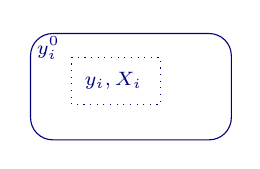
\begin{tikzpicture}[scale=0.75,NavyBlue]
  \draw[rounded corners=8pt] (0,0) rectangle (3.4,1.8);
  \draw[dotted] (0.7,0.6) rectangle (2.2,1.4);
  \node at (1.4,1.0) {\scriptsize $y_i, X_i$};
  \node at (0.3,1.55) {\scriptsize $y_i^0$};
\end{tikzpicture}
{\scriptsize v rovn.\ $y_i = y_i^0\ \forall_i$ \\
$\bullet$ fluktuace: $X_i\to X_i + \delta X_i^f$ $\leftarrow$ fluktuace \\
$\Rightarrow \delta y_i^f = \left(\frac{\partial y_i}{\partial X_i}\right)\delta X_i^f$ \dots\ prim.\ efekt \\
\phantom{$\Rightarrow$} $\delta y_j^f = \left(\frac{\partial y_j}{\partial X_i}\right)\delta X_i^f$ \dots\ sekund.\ efekt}
\end{minipage}

\begin{itemize}[nosep]
  \item pracujeme v $S = S(U,V)$ repre, systém v kontaktu s $T_0, p_0$
  \item proces zpět do rovnováhy: \quad $\delta U^r = -\delta U_0^r$, \ $\delta V^r = -\delta V_0^r$ \qquad $r$ \dots\ response
\end{itemize}
\[
  \dd S_{tot} = \left(\frac1T - \frac{1}{T_0}\right)\delta U^r + \sum_{i=1}^{k}\left(\frac{y_i}{T} - \frac{y_{i,res}}{T_0}\right)\delta X^r \geq 0
\]
\[
  \text{spec.}\quad \left(\frac1T - \frac{1}{T_0}\right)\delta U^r + \left(\frac{p}{T} - \frac{p_0}{T_0}\right)\delta V^r \geq 0
\]
\[
  \frac1T - \frac{1}{T_0} = \frac{1}{T_0 + \delta T^f} - \frac{1}{T_0} \simeq -\frac{\delta T^f}{T_0^2}
\]
\[
  \frac{p_0 + \delta p^f}{T_0 + \delta T^f} - \frac{p_0}{T_0} = \frac{T_0p_0 + T_0\delta p^f - T_0p_0 - \delta T_f\,p_0}{T_0^2}
  = \frac{\delta p_f}{T_0} - \frac{p_0}{T_0^2}\delta T_f
\]
\[
  \Rightarrow\ -\frac{1}{T_0}\delta T^f\delta U^r + \delta p^f\delta V^r - \frac{p_0}{T_0}\delta T^f\delta V^r \geq 0
\]
\[
  \Leftrightarrow\ -\delta T^f\delta S^r + \delta p^f\delta V^r \geq 0
  \quad\Leftrightarrow\quad \fbox{$\delta T^f\delta S^r - \delta p^f\delta V^r \leq 0$}
\]
\begin{itemize}
  \item $\delta V^r, \delta S^r$ jsou nezávislé \dots\ proces do rovnováhy může být buď skrze $\dbar Q$ nebo $\dbar W$
\end{itemize}
$\Rightarrow$ \underline{primární odezva}: \fbox{$\delta p^f\delta V^r \geq 0$}
\begin{itemize}
  \item[] $\bullet$ \ $\delta p^r = \left(\pdv{p}{V}\right)_S\delta V^r = \dfrac{V}{V}\left(\pdv{p}{V}\right)_S\delta V^r = -\dfrac{1}{V\kappa_S}\delta V^r$
  \[
    \Rightarrow\ \delta V^r = -V\kappa_S\,\delta p^r \ \Rightarrow\ -V\kappa_S\,\delta p^f\delta p^r \geq 0
    \ \overset{\kappa_S\geq0}{\Rightarrow}\ \fbox{$\delta p^f\delta p^r \leq 0$}\ \textcolor{OliveGreen}{\checkmark}
  \]
\end{itemize}
$\Rightarrow$ \underline{sekundární odezva}: \fbox{$\delta T^f\delta S^r \leq 0$}
\[
  \delta T^f = \left(\pdv{T}{V}\right)_S\delta V^f = -\left(\pdv{T}{V}\right)_S\kappa_SV\,\delta p^f
\]
\[
  \Rightarrow\ \delta T^f\delta S^r = -\left(\pdv{T}{V}\right)_S\kappa_SV\,\delta p^f\delta S^r
  = \Big/\ -\left(\pdv{T}{V}\right)_S = \left(\pdv{p}{S}\right)_V\ \Big/
\]
\[
  = \kappa_SV\,\delta p^f\delta p^r \leq 0 \ \Rightarrow\ \fbox{$\delta p^f\delta p^r \leq 0$}\ \textcolor{OliveGreen}{\checkmark}
\]
\begin{itemize}
  \item stabilitu jsme využili 2$\times$: \quad 1) $\dd S_{tot} \geq 0$ v procesu do rovnováhy \\
        \hspace*{4.3cm} 2) $\kappa_S \geq 0$
  \item a co jako celek: \quad $\delta T^f\delta S^r - \delta p^f\delta V^r = \kappa_SV\delta p^f\delta p^r + \kappa_SV\delta p^f\delta p^r = 2\kappa_SV\delta p^f\delta p^r \leq 0$ \\
        $\Rightarrow$ lze to také!
\end{itemize}
\endgroup

%----------------------------------------------------------------------
\strana{L6b-12}
\begingroup\color{NavyBlue}
\begin{itemize}
  \item jak je to v řeči ext.\ veličin:
  \[
    \delta p^f = \left(\pdv{p}{V}\right)_S\delta V^f \ \Rightarrow\ \delta V^f > 0 \ \Rightarrow\ \delta p^f < 0
    \ \Rightarrow\ \big/\ \delta p^f\delta V^r \geq 0\ \big/ \ \Rightarrow\ \delta V^r < 0 \ \checkmark
  \]
  $\Rightarrow$ píst se vrací do původní polohy
\end{itemize}
\begin{center}\rule{0.4\linewidth}{0.4pt}\end{center}
\[
  \delta T^f = \left(\pdv{T}{V}\right)_S\delta V^f = -\frac{\left(\pdv{S}{V}\right)_T}{\left(\pdv{S}{T}\right)_V}\delta V^f
  = \big/\ \dd F = -S\,\dd T - p\,\dd V\ \big/ = -\frac{T\left(\pdv{p}{T}\right)_V}{C_V}\delta V^f
\]
\[
  = \frac{T\left(\pdv{V}{T}\right)_p}{C_V\left(\pdv{V}{p}\right)_T}\delta V^f
  = \fbox{$-\dfrac{T\alpha}{C_V\kappa_T}\delta V^f = \delta T^f$}
  \qquad \delta T^f \gtrless 0 \ \text{(znam.\ $\alpha$ neznám)}
\]
\[
  \Rightarrow\ -\frac{T\alpha}{C_V\kappa_T}\delta V^f\delta S^r = -\frac{\alpha}{C_V\kappa_T}\delta V^f\delta Q^r \leq 0
  \ \Leftrightarrow\ \fbox{$\alpha\,\delta V^f\delta Q^r \geq 0$}
\]
\[
  \Rightarrow\ \Big/\ \alpha\,\delta V^f = -\frac{C_V\kappa_T}{T}\delta T^f\ \Big/ \ \Rightarrow\ \delta T^f\delta Q^r \leq 0
  \ \dots\ \text{což je samozřejmě původní } \delta T^f\delta S^r \leq 0
\]
\begin{tabular}{@{}ll}
neboli: & $T\nearrow\ S\searrow$ ($Q$ odtéká) \\
        & $T\searrow\ S\nearrow$ ($Q$ přitéká)
\end{tabular}
\quad \dots\ tok tepla vyrovnává změnu teploty a tedy změnu tlaku

\begin{itemize}
  \item obecně $\delta X$ vyvolá nehomogenity v int.\ proměnných \\
        $\Rightarrow$ stabilita systému je vyhlazuje
  \item LChB $\to$ znaménka koef.\ lin.\ odezvy? Zde dostáváme $\kappa_S > 0$ (za předp., že je $\kappa_S\neq0$, jinak to celé spadne)
\end{itemize}
\endgroup

%----------------------------------------------------------------------
\strana{L6b-13}
\begin{priklad}[Př:]
\begin{minipage}{0.55\textwidth}
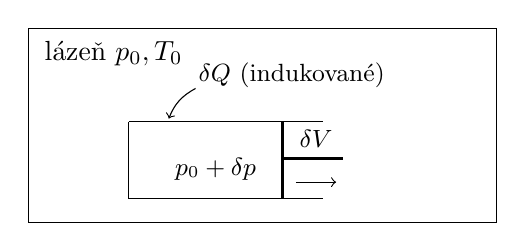
\begin{tikzpicture}[scale=0.85]
  \draw (0,0) rectangle (7,2.9);
  \node[anchor=north west] at (0.1,2.85) {lázeň $p_0, T_0$};
  % válec
  \draw (1.5,0.35) -- (4.4,0.35);
  \draw (1.5,0.35) -- (1.5,1.5);
  \draw (1.5,1.5) -- (4.4,1.5);
  \draw[very thick] (3.8,0.35) -- (3.8,1.5);
  \draw[very thick] (3.8,0.95) -- (4.7,0.95);
  \node at (2.8,0.8) {\small $p_0 + \delta p$};
  \node at (4.3,1.25) {\small $\delta V$};
  \draw[->] (4.0,0.6) -- (4.6,0.6);
  \node[anchor=west] at (2.4,2.2) {\small $\delta Q$ (indukované)};
  \draw[->] (2.5,2.0) to[bend right=20] (2.1,1.55);
\end{tikzpicture}
\end{minipage}
\begin{minipage}{0.43\textwidth}
$\bullet$ píst se pohne ven \\
$\delta V > 0 \Rightarrow \delta p < 0 \Rightarrow$ primární efekt je mech.\ vyrovnání tlaků zpětným poklesem $V$ (Le-Chatelier)
\end{minipage}

\begin{itemize}
  \item sekundární efekt je pokles teploty:
  \[
    \delta T = \left(\pdv{T}{V}\right)_S\delta V
    = -\frac{T\left(\pdv{S}{V}\right)_T}{T\left(\pdv{S}{T}\right)_V}\delta V = -\frac{T\left(\pdv{p}{T}\right)_V}{C_p}\delta V
  \]
  \cervene{\small $\uparrow$ ($S$) adiabaticky, neboť výše zakreslený tok tepla je až sekundární}
  \[
    \Rightarrow\ \delta T = -\frac{T\alpha}{C_p\kappa_T}\delta V
  \]
  \item protože znaménko $\alpha$ neznáme, $\delta T$ může být kladné i záporné
  \item $\delta T$ vyvolá tok tepla $\delta Q \propto \operatorname{sign}\alpha$ \ ($\delta Q > 0$ je teplo do podsystému)
  \item změna tlaku indukovaná tímto tokem tepla je
  \[
    \underset{\substack{\nearrow\\ \modre{\text{LChB}}}}{\modre{0\leq}}\ \delta p = \left(\pdv{p}{S}\right)_V\frac{\delta Q}{T}
    = \frac1T\left(\pdv{p}{T}\right)_V\left(\pdv{T}{S}\right)_V\delta Q
  \]
  \[
    = -\frac{1}{C_V}\frac{\left(\pdv{V}{T}\right)_p}{\left(\pdv{V}{p}\right)_T}\delta Q
    = \frac{\alpha}{C_V\kappa_T}\delta Q \propto \frac{|\alpha|}{C_V\kappa_T} > 0
  \]
  \hspace*{2cm}$\Rightarrow$ tok tepla také indukuje růst tlaku
\end{itemize}
$\Rightarrow$ \kw{oba indukované procesy vedou k návratu do rovnováhy, jak tvrdí LChB princip}
\end{priklad}

%----------------------------------------------------------------------
\strana{L6b-14}
\begingroup\color{Red}
\begin{itemize}
  \item primární/sekundární odkazuje na změnu sdružené/jiné intenzivní proměnné
\end{itemize}
\[
  \underset{\substack{\updownarrow\\ \text{vynucená změna}}}{X_1\to X_1 + \delta X_1^f}
  \ \Rightarrow\
  \begin{aligned}
    \delta y_1 &= \left(\pdv{y_1}{X_1}\right)\delta X_1 && \dots\ \text{prim.\ efekt} \\
    \delta y_2 &= \left(\pdv{y_2}{X_1}\right)\delta X_1 && \dots\ \text{sek.\ efekt}
  \end{aligned}
\]
\begin{itemize}
  \item změny $\delta y_i$ indukují $\delta X_i^r$ (response), které směřují k rovnováze $\Leftrightarrow$ pokles $U$
  \[ \delta U^r = \delta y_1\,\delta X_1^r + \delta y_2\,\delta X_2^r \leq 0 \]
  \item $\delta X_1^r$ a $\delta X_2^r$ nezávislé (mohu lib.\ $X_i$ fixovat a stále vztah platí)
\end{itemize}
\[
  \Rightarrow\ \text{i)}\ \left(\pdv{y_1}{X_1}\right)\delta X_1^f\delta X_1^r \leq 0
  \qquad \Big/\cdot\left(\pdv{y_1}{X_1}\right) \geq 0 \Leftarrow \text{konvexita } U
\]
\[
  \Rightarrow\ \delta y_1^f\,\delta y_1^r \leq 0 \quad \Leftrightarrow\ \text{\parbox[t]{6cm}{indukovaná změna má opačné znaménko než vynucená}}
\]
\[
  \text{ii)}\ \left(\pdv{y_2}{X_1}\right)\delta X_1^f\delta X_2^r = \Big/\ \left(\pdv{y_2}{X_1}\right) = \left(\pdv{y_1}{X_2}\right)\ \Big/
\]
\[
  = \delta X_1^f\left[\left(\pdv{y_1}{X_2}\right)\delta X_2^r\right] \leq 0 \qquad \Big/\cdot\left(\pdv{y_1}{X_1}\right) \geq 0
\]
\[
  \Rightarrow\ \delta y_1^f\cdot\delta y_1^r \leq 0
\]
$\Rightarrow$ v obou případech jde indukovaná variace proti vynucené, tedy vyrovnává nehomogenitu -- v souladu s LChB pr.
\endgroup

